Task B1 is to implement a system call. This is a pretty fundamental feature in operating systems.\\

When designing an operating system you will soon run into thoughts about security. How would you secure that only system related activities
can access the system's resources directly? Easy, some might say. Just divide it into two areas with different privilege level. 
In operating systems those two levels are called user- and kernel mode. Not all operating systems have this split, but if you have a
 lot of 3rd party development you ought to make this split.\\
Programs running in kernel mode have direct access to all I/O devices, memory and so forth. This gives a lot of possibilities (-to mess something up).\\
Programs running in user mode do not have the same privileges and need therefore to have some kind of service specified in order to communicate with I/O and get extra memory. This ``API'' is called system calls. System calls are a set of commands that the operating system listens for and when these are called the system supplies the caller with the service applied for.\\
When a syscall is invoked, the CPU registers is pushed on the stack and the OS switches to kernel mode. The kernel uses a macro that calls some low-level assembler code in order to achieve this.


\begin{figure}
\centering
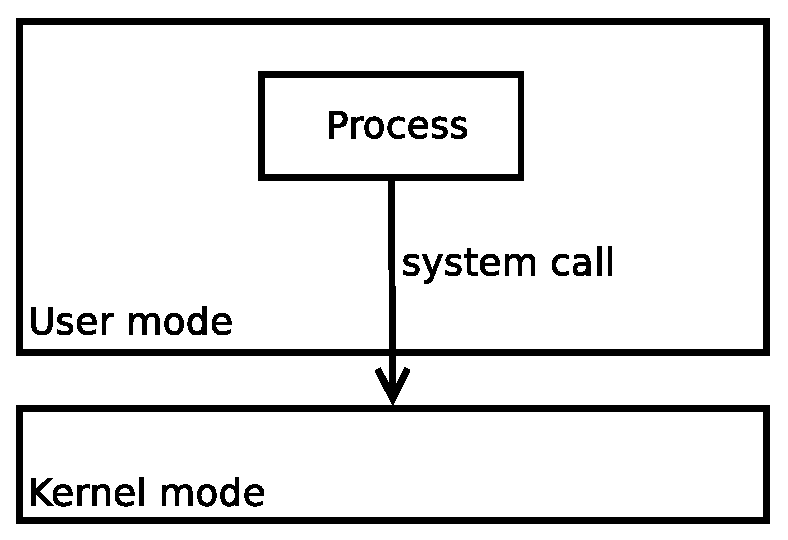
\epsfig{file=fig/Kernel_Mode.eps, height=1in}
\caption{Invoking a system call}
\label{fig:kernel_mode}
\end{figure}

\subsection{Reflections}

\subsubsection*{What kind of operating system is it?}
Tanenbaum and Woodhull describes three major types of operating system kernel types; monolithic, mico and exo.\\
The microkernel is based on the design philosophy that everything is implemented as a service, meaning that things like process management is done
in userspace and these services communicate via an IPC scheme (see section \ref{sec:ipc}).\\
%The exokernel is type of kernel that serves as a kernel on top other kernels in a hypervisor way\\
The monolithic kernel is proportionally weak in design pattern as microkernels is strong. They pretty much go by the ``anything goes'' design 
strategy. Our system is a monolithic operating system. Nothing is implemented as a service as in a microkernel or takes on any of the
characteristics of an exokernel.

%Draw a figure of the organization of the system. Relate the organization of the system to the different types of operation systems discussed in the text book by Tanenbaum and Woodhull. What kind of operating system is it?  Why?

\subsubsection*{Which portion execute in kernel mode? Which portions in user mode? What is the difference between user and kernel mode?}
All system calls is run in kernel mode. The kernel mode has access to system resources user mode doesn't

\subsubsection*{How is the kernel invoked from the user-level program? Explain and elaborate!}
The kernel is invoked through system calls. When a syscall is invoked, the CPU registers is pushed on the stack and switches to kernel mode. The kernel uses a macro that calls some low-level assembler code.

\subsubsection*{How is control passed back to the user-level program? Explain and elaborate!}

When the syscall returns, the stack is pushed back into the registers and the computer returns to user mode and continues the execution of the
program that did the system call.

\subsection{Test}
The executing program is to make the system call\\ “SYSCALL\_VERSION” where the kernel version should be printed to the bochs console. This desired result was achieved as defined in task definition, and the test was a success.